\chapter{Attribute prediction for retail sector products} % (fold)
\label{cha:attribute_prediction_for_retail_sector_products}

\section{Introduction} % (fold)
\label{sec:introduction}

Goals.
Context: NLP challenges.
Approaches.
Encountered challenges. 

\section{Text Classification} % (fold)
\label{sec:}

\subsection{NLP challenge: word representation}


\subsubsection{CBOW}

\subsubsection{Skip-Gram}

\begin{figure}
  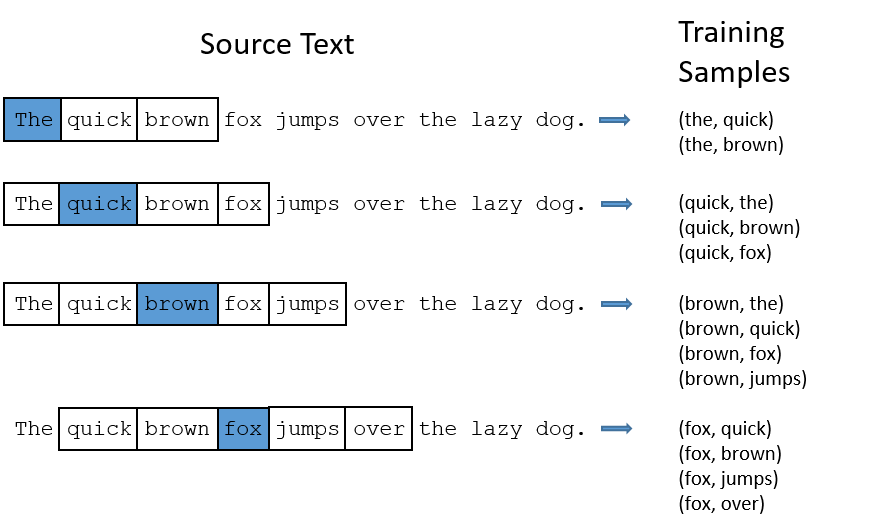
\includegraphics[width=\linewidth]{images/skip-gram.png}
  \caption{Text sample}
  \label{fig:sample}
\end{figure}

We start by briefly reviewing the continuous skipgram model introduced by \newcite{mikolov2013distributed}, from which our model is derived.
Given a word vocabulary of size $W$, where a word is identified by its index $w~\in~\{1, ..., W\}$, the goal is to learn a vectorial representation for each word $w$.
Inspired by the distributional hypothesis~\cite{harris1954distributional}, word representations are trained to \emph{predict well} words that appear in its context.
More formally, given a large training corpus represented as a sequence of words $w_1, ..., w_T$, the objective of the skipgram model is to maximize the following log-likelihood:
\begin{equation*}
  \sum_{t=1}^T \ \sum_{c \in \mathcal{C}_t} \ \log p(w_c \ | \ w_t),
\end{equation*}

where the context $\mathcal{C}_t$ is the set of indices of words surrounding word $w_t$.

The probability of observing a context word $w_c$ given $w_t$ will be parameterized using the aforementioned word vectors.
For now, let us consider that we are given a scoring function~$s$ which maps pairs of (word, context) to scores in~$\mathbb{R}$.
One possible choice to define the probability of a context word is the softmax:
\begin{equation*}
p(w_c \ | \ w_t) = \frac{e^{s(w_t,\ w_c)}}{\sum_{j=1}^W e^{s(w_t,\ j)}}.
\end{equation*}
However, such a model is not adapted to our case as it implies that, given a word $w_t$, we only predict one context word $w_c$.

The problem of predicting context words can instead be framed as a set of independent binary classification tasks.
Then the goal is to independently predict the presence (or absence) of context words.
For the word at position $t$ we consider all context words as positive examples and sample negatives at random from the dictionary.

Probability that word $w_c$ is in context of $w_t$:
\begin{align*}
	p(w_c | w_t) &= \frac{e^{s(w_t, w_c)}}{\sum_{n \in N_{t,c}} e^{s(w_t, n)}} 
%	p(w_c | w_t) &= \frac{1 + e^{- s(w_t, w_c)}}{1 + \sum_{n \in N_{t,c}} e^{s(w_t, n)}}

\end{align*}

Notes:
\begin{align*}
  \sum_{j=1}^W p(w_j | w_t) &= \sum_{j=1}^W \frac{e^{s(w_t, w_j)}}{\sum_{n \in N_{t,j}} e^{s(w_t, n)}} \\
  \sum_{j=1}^W p(w_j | w_t) &> \sum_{j=1}^W \frac{e^{s(w_t, w_j)}}{\sum_{j=1}^W e^{s(w_t, w_j)}} \\
  \sum_{j=1}^W p(w_j | w_t) &> 1 
\end{align*}

For a chosen context position $c$, using the binary logistic loss, we obtain the following negative log-likelihood:
\begin{equation*}
  \log \left(1 + e^{-s(w_t,\ w_c)} \right) + \sum_{n \in \mathcal{N}_{t, c}} \log \left(1 + e^{s(w_t,\ n)}\right),
\end{equation*}
where $\mathcal{N}_{t,c}$ is a set of negative examples sampled from the vocabulary.
By denoting the logistic loss function $\ell: x \mapsto \log(1 + e^{-x})$, we can re-write the objective as:
\begin{equation*}
\sum_{t=1}^{T}  \left [ \sum_{c \in \mathcal{C}_t} \ell(s(w_t,\ w_c)) + \sum_{n \in \mathcal{N}_{t,c}} \ell(-s(w_t,\ n)) \right ].
\end{equation*}




We are looking for the similarity function $s$ that maximize the log likelyhood.
\begin{equation*}
	\hat s \in argmax_{s\in S} \sum_{t=1}^{T}  \left [ \sum_{c \in \mathcal{C}_t} \ell(s(w_t,\ w_c)) + \sum_{n \in \mathcal{N}_{t,c}} \ell(-s(w_t,\ n)) \right ]
\end{equation*}




A natural parameterization for the scoring function $s$ between a word $w_t$ and a context word $w_c$ is to use word vectors.
Let us define for each word $w$ in the vocabulary two vectors $u_w$ and $v_w$ in $\mathbb{R}^d$.
These two vectors are sometimes referred to as \emph{input} and \emph{output} vectors in the literature.
In particular, we have vectors $\mathbf{u}_{w_t}$ and $\mathbf{v}_{w_c}$, corresponding, respectively, to words $w_t$ and $w_c$.
Then the score can be computed as the scalar product between word and context vectors as $s(w_t, w_c) = \mathbf{u}_{w_t}^{\top} \mathbf{v}_{w_c}$.
The model described in this section is the skipgram model with negative sampling, introduced by \newcite{mikolov2013distributed}.

We are looking for the \emph{input} and \emph{output} vectors $U$, $V$ that maximize the log likelyhood:
\begin{equation*}
	(\hat U, \hat V) \in argmax_{U \in M_{(|W|, d)}, V \in M_{(d, |W|)} } \sum_{t=1}^{T}  \left [ \sum_{c \in \mathcal{C}_t} \ell(\mathbf{u}_{w_t}^{\top} \mathbf{v}_{w_c}) + \sum_{n \in \mathcal{N}_{t,c}} \ell(-\mathbf{u}_{w_t}^{\top} \mathbf{v}_{n}) \right ]
\end{equation*}


\subsection{Subword model}
\label{sec:model-ngrams}

By using a distinct vector representation for each word, the skipgram model ignores the internal structure of words.
In this section, we propose a different scoring function $s$, in order to take into account this information.

Each word $w$ is represented as a bag of character $n$-gram.
We add special boundary symbols \texttt{<} and \texttt{>} at the beginning and end of words, allowing to distinguish prefixes and suffixes from other character sequences.
We also include the word $w$ itself in the set of its $n$-grams, to learn a representation for each word (in addition to character $n$-grams).
Taking the word \emph{where} and $n=3$ as an example, it will be represented by the character $n$-grams:
\begin{center}
\texttt{<wh, whe, her, ere, re>}
\end{center}
and the special sequence
\begin{center}
\texttt{<where>}.
\end{center}
Note that the sequence \texttt{<her>}, corresponding to the word \emph{her} is different from the tri-gram \texttt{her} from the word \emph{where}.
In practice, we extract all the $n$-grams for $n$ greater or equal to 3 and smaller or equal to $6$.
This is a very simple approach, and different sets of $n$-grams could be considered, for example taking all prefixes and suffixes.

Suppose that you are given a dictionary of $n$-grams of size $G$.
Given a word $w$, let us denote by $\mathcal{G}_w \subset \{1, \dots, G \}$ the set of $n$-grams appearing in $w$.
We associate a vector representation $\mathbf{z}_g$ to each $n$-gram $g$.
We represent a word by the sum of the vector representations of its $n$-grams.
We thus obtain the scoring function:
\begin{equation*}
s(w, c) = \sum_{g \in \mathcal{G}_w} \mathbf{z}_g^\top \mathbf{v}_c.
\end{equation*}
This simple model allows sharing the representations across words, thus allowing to learn reliable representation for rare words.

In order to bound the memory requirements of our model, we use a hashing function that maps $n$-grams to integers in 1 to $K$.
We hash character sequences using the Fowler-Noll-Vo hashing function (specifically the \texttt{FNV-1a} variant).\footnote{\smaller\relax\url{http://www.isthe.com/chongo/tech/comp/fnv}}
We set $K = 2.10^6$ below.
Ultimately, a word is represented by its index in the word dictionary and the set of hashed $n$-grams it contains.





\subsubsection{CBOW model}

\subsubsection{Fasttext model}

\subsection{Multilabel challenge}

\section{POS tagging} % (fold)
\label{sec:}

% section sampling (end)

\section{Evaluation} % (fold)
\label{sec:evaluation}

% section evaluation (end)

% chapter churn_prediction_in_the_FMCG_retail_sector (end)
